% This is LLNCS.DEM the demonstration file of
% the LaTeX macro package from Springer-Verlag
% for Lecture Notes in Computer Science,
% version 2.4 for LaTeX2e as of 16. April 2010
%
\documentclass{llncs}
%
\usepackage{indentfirst}
\usepackage{makeidx}  % allows for indexgeneration
\usepackage{algpseudocode}
\usepackage{multirow}
\usepackage{longtable}
\usepackage{amsmath}
\usepackage{algorithm}
\usepackage{algorithmic}
\usepackage{amsfonts,dsfont}
\usepackage{graphicx}

\begin{document}
\title{Training Deep Nets with Progressive Batch Normalization on multi-GPUs}

% \author{Lianke Qin \inst{1}, Yifan Gong \inst{1} , Tianqi Tang \inst{1} , Yutian Wang  \inst{2} ,Jiangming Jin \inst{1}}  
% \institute{Tusimple \and Computer Science Department, Tsinghua University}
\author{}
\institute{}
\maketitle

\begin{abstract}
Batch Normalization(BN) enables us to train various deep neural networks faster. However, the training accuracy will be significantly influenced with the decrease of input mini-batch size. 
To increase the model accuracy, a global mean and variance
among all the input batch can be used, nevertheless communication
across all devices is required in each BN layer, which reduces the
training speed greatly.
To address this problem, we propose Progressive Batch Normalization (PBN), which can achieve a good balance between model accuracy and efficiency in multiple-GPU training. Experimental results show that our algorithm can obtain significant performance improvement over traditional BN without data synchronization across GPUs, achieving up to 18.4\% improvement on training DeepLab for semantic segmentation task across 8 GPUs.
\end{abstract}

\begin{keywords}
Batch normalization, Data parallelism, Deep learning
\end{keywords}
\section{Introduction}

Deep neural networks have achieved significant success in many domains in recent years, such as speech recognition, visual object recognition, and text processing. To meet more and more complicated deep learning applications, neural networks go deeper and wider. However, as both memory and computational cost increase with the depth and width of network linearly, data parallelism across multiple devices is deployed to accelerate the process of model training.

To accelerate deep network training, \emph{Batch Normalization (BN)}~\cite{ioffe2015batch} is proposed. Through making normalization as a part of the model architecture and performing the normalization for each sub mini-batch, BN allows developers to use much higher learning rates to improve the rate of model convergence. In a conventional BN layer, the mean and variance of parameter values are calculated only within a sub mini-batch on a given device. In this way, the main advantage is that cross-device communications are not necessary during the training process. However, as the decrease of input mini-batch size, the training accuracy will be significantly influenced by this means. Therefore, the training accuracy could be greatly hurt when few images can be put in a single GPU due to memory limitation and large image size.


% Taking the deep learning model used in self-driving as an example. only 3 images can be put in a single GPU in semantic segmentation training for ResNet-50 with cityscapes dataset due to memory limitation. As a result, the training accuracy could be greatly hurt under the conventional BN algorithm due to a limited input image size. 

To increase the model accuracy, a global mean and variance among all the input batch can be introduced, nevertheless communication across all devices is required in each BN layer, which reduces the training speed greatly. Based on our observation for different deep network training, the training accuracy increases with input batch size generally while there exists a threshold under which the quality of model will be deteriorated. Therefore, for a large batch size, such as imagenet~\cite{krizhevsky2012imagenet}, the training accuracy loss resulting from local mean and variance is negligible compared to the introduced communication cost. However, when to select a local or a global Batch Normalization to achieve a good balance between model accuracy and training speed is very challenging for most model developers.  

To address the above challenge, we propose a novel technique, called Progressive Batch Normalization (PBN), which can achieve a good balance between accuracy and efficiency in multiple GPUs. In PBN, variables such as mean and variances are calculated based on the data across the whole devices to realize complete data parallelism. We implement our algorithm in a production deep learning framework, MXNet~\cite{chen2015mxnet}. Experimental results show that 
our algorithm can get up to 18.4\% performance improvement over traditional methods without sacrificing the training accuracy. 


\section{Preliminary and Background}

\subsection{Data parallelism}


Recently, many advances in deep neural network training involve in fitting large models to massive datasets in order to achieve good results. But training deep network is time-consuming with data size increasing and model parameters expanding. Distributed implementation partition training data and store it across multiple-GPUs~\cite{data-parallelism}. We call this data-parallelism.   


\begin{figure}[h]
\begin{minipage}[t]{0.45\linewidth}
\centering
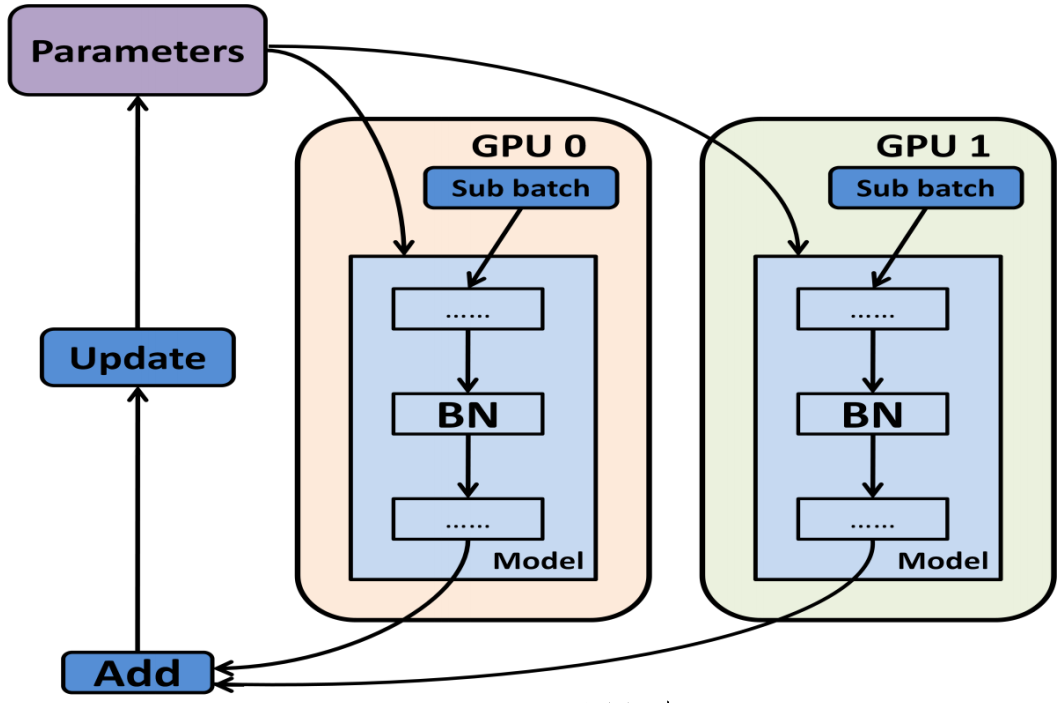
\includegraphics[width=1\textwidth]{figure/noreduce.png}
    \caption{Data parallelism in batch normalization layer}%
    \label{fig:localBN}
\end{minipage}
\hfill
\begin{minipage}[t]{0.45\linewidth}
\centering
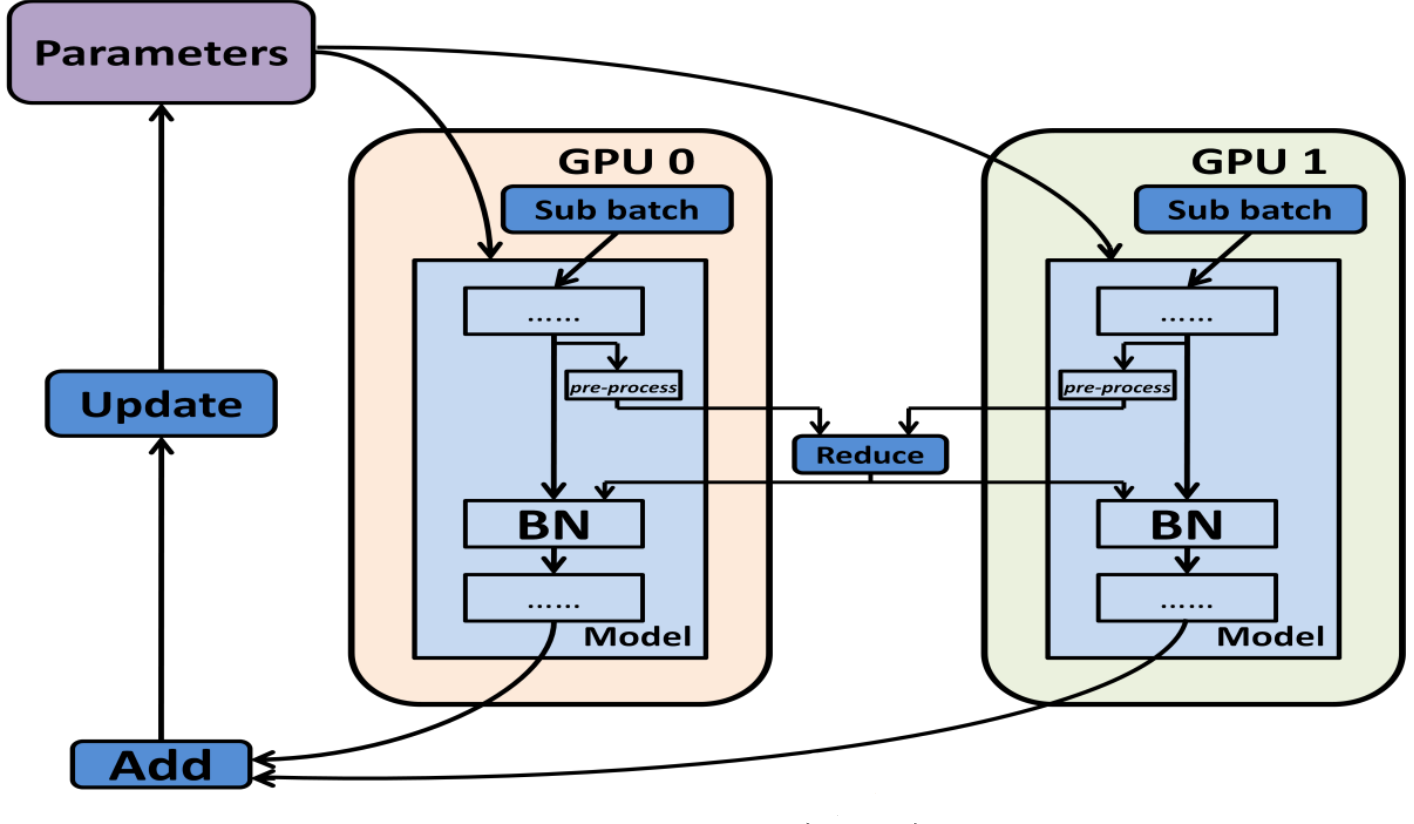
\includegraphics[width=1\textwidth]{figure/reduce.png}
    \caption{Schematic of the process of global BN operator }
    \label{fig:globalBN}
\end{minipage}
\end{figure}

\subsection{Batch Normalization}

The distribution of each layer's inputs varies during the training process. We used to be careful about parameter initialization and lowering learning rate. Batch Normalization\cite{ioffe2015batch} was put forward to solve this \textit{interval covariate shift} phenomenon. The idea is to normalize the inputs to layers within the network and apply a transformation that makes the mean close to 0 and standard deviation close to 1. Batch Normalization brings those benefits : network training faster, higher learning rate, easier weights initialization, etc. Figrue~\ref{fig:localBN} shows the Batch Normalization in data parallelism.



\subsection{Global Batch Normalization}

Taking the forward propagation of BN layer as an example, the original
BN algorithm consists of only one section: normalization. 
In Global Batch Normalization as shown in Figure~\ref{fig:globalBN}, we add two sections, pre-pocessing and
reduce, to adjust the normalization section accordingly.


In the pre-pocessing section, we compute the \textbf{local} mean and square of mean, here \textbf{local} means the output is computed from the data on the $i$th GPU, $m_i$ indicates the mini-batch size of the $i$th GPU. 
\begin{equation}
\label{equ:prepocessing}
\left\{ {\begin{array}{*{20}{c}}
{{u_i} = \frac{1}{{{m_i}}}\sum\limits_{j = 1}^{{m_i}} {{x_{i,j}}} }\\
{{v_i} = \frac{1}{{{m_i}}}\sum\limits_{j = 1}^{{m_i}} {x_{i,j}^2} }
\end{array}} \right.
\end{equation}

In reduce section, we compute the global mean and square of mean, and \textbf{global} means the output is based on the data of whole devices as shown in Equation~\ref{equ:reduce}. $n$ indicates the count of devices.
\begin{equation}
\label{equ:reduce}
\left\{ {\begin{array}{*{20}{c}}
{u = \frac{{\sum\nolimits_{i = 1}^n {{u_i}{m_i}} }}{{\sum\nolimits_{i = 1}^n {{m_i}} }}}\\
{v = \frac{{\sum\nolimits_{i = 1}^n {{v_i}{m_i}} }}{{\sum\nolimits_{i = 1}^n {{m_i}} }}}
\end{array}} \right.
\end{equation}

The normalization section is similar to the original BN algorithm except the operation of getting global variance, and the output is identical to the original BN algorithm if the reduce section is ignored as shown in Equation~\ref{equ:normalization}.
\begin{equation}
\label{equ:normalization}
\left\{ {\begin{array}{*{20}{c}}
{{\sigma ^2} = v - {u^2}}\\
{{{\hat x}_{i,j}} = \frac{{{x_{i,j}} - u}}{{\sqrt {{\sigma ^2} + \varepsilon } }}}\\
{{y_{i,j}} = \gamma {{\hat x}_{i,j}} + \beta }
\end{array}} \right.
\end{equation}

When training mini batch size is too small, using global batch normalization layer can improve validation accuracy a lot.


\section{Observation}

We evaluate the training accuracy and performance of Global BN algorithm under different batch size $B$. 
%We denote the batch size as $B$ for the whole devices, and the batch size in a single device $B_{sub}=B/N$, where $N$ indicates the count of devices. 
We divide all the GPUs into groups of different size,
and only let GPUs from the same group share their batch normalization layer's key data. 
We vary the group size from 1 to 8.
We utilize Resnet-20 model based on Cifa10 dataset as an example.


\subsection{Accuracy improvement}

\begin{figure}[h]
\begin{minipage}[t]{0.45\linewidth}
\centering
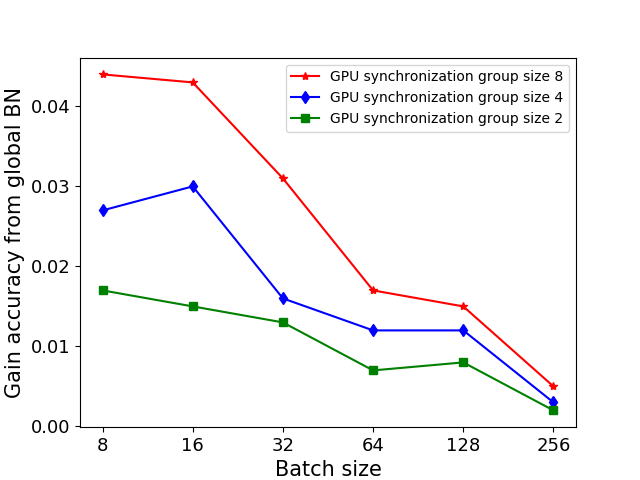
\includegraphics[width=1\textwidth]{figure/cifar10-gain.png}
\caption{Training accuracy gain in different group size}
\label{fig:accVsBz}
\end{minipage}
\hfill
\begin{minipage}[t]{0.45\linewidth}
\centering
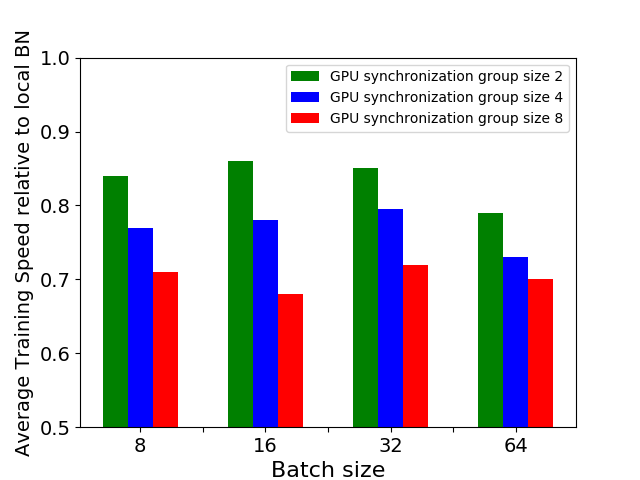
\includegraphics[width=1\textwidth]{figure/cifar10-speedloss.png}
\caption{Training speed loss in different group size}
\label{fig:speedloss}
\end{minipage}
\end{figure}


%As we can see, 
We have two observations from Figure~\ref{fig:accVsBz}. First, for the fixed batch size $B$, the training accuracy increases as we vary the group size from 1 to 8. For 
the batch size $B$=8, the training accuracy raises up to \textbf{4.4\%} when synchronization group size is 8. 
%When we vary the group size to 2 or 4, the accuracy improvement is less effective. 
%but the smaller the group is, the less extra time the synchronization process costs. 
%Results are shown in Figure~\ref{fig:accVsBz}. 
Second, 
%It is clear that 
the accuracy earning from data synchronization during batch normalization decreases monotonously as batch size grows. This is reasonable because when batch size in each group is large enough, 
the local optimal solution is near the global optimal solution.
%the optimization method Stochastic Gradient Descent can find nearly the best direction to minimize loss, and combining these mini batches into one has little effect on the performance of SGD.



\subsection{Speed Loss}


% \begin{figure}
% \centering
% 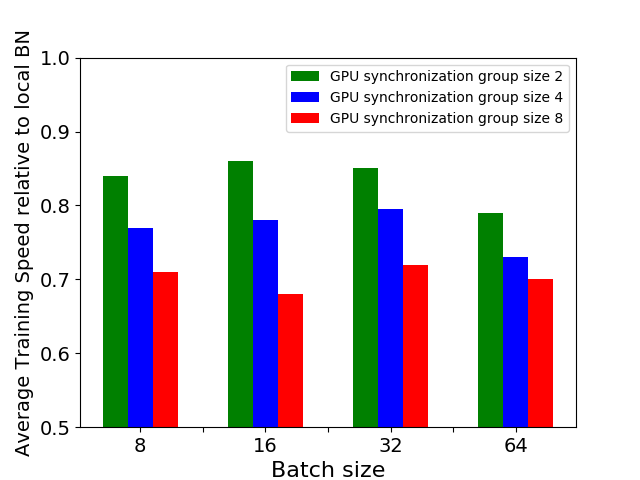
\includegraphics[width=6cm]{figure/cifar10-speedloss.png}
% \caption{Speed loss from Global BN compared to Local BN}
% \label{fig:speedloss}
% \end{figure}

As we all know, we have to train a deep neural network for many epochs to make it converge, which means that communication overhead between GPUs in Global BN algorithm can not be ignored. Figure~\ref{fig:speedloss} shows 
the average training speed per epoch
%how much time it takes to train one epoch on average 
%on Cifar10 dataset with Resnet-20 
under different synchronization group sizes compared to traditional BN.
We observe that the overhead from data synchronization across all devices occupies around \textbf{30\%} of the total time of Global BN algorithm in most cases. 
We also observe that the total overhead reduces as the group size decreases.
%As the group size  
%Such high overhead from communication when training deep neural network exceeds what we can bear. We will propose several practical strategies to reduce it to an affordable range later.


\subsection{Motivation}
Theoretically speaking, the smaller the group is, the lower extra cost from stragglers is. But accuracy gain from synchronization reduces accordingly, too.
Based on the observations, we find that there is a trade-off between accuracy improvement and speed loss.
Like hierarchy design in other areas, synchronization across GPUs can also be based on it. We can divide 8 GPUs into 2 or 4 groups and synchronization only take place with groups separately. In other words, there is an opportunity in determining the synchronization group size to optimize the performance and training accuracy.



\section{Progressive Batch Normalization}


%\subsection{Model Overview}


\subsection{Problem Formulation}


Consider a traditional deep neural network training process with $N$ GPUs. The training process is divided into several epochs.
In epoch $i$, we evaluate the accuracy $A_i$ and determine how many GPUs will share data with each other as a group, we denote the number of GPUs in each group as $X_i$. 
We further calculate the accuracy improvement $\delta_{A_i}(X_i)$ in epoch $i$, where $\delta_{A_i}(X_i)$=$A_i$-$A_{i-1}$.
The training time is denoted as $t(X_i)$, which is fixed when $X_i$ is given. The training process will stop until the accuracy reaches to a given accuracy $A_{max}$.


\begin{table}[]
    \centering
    \begin{tabular}{|c|c|}
        \hline    Name & Description  \\
        \hline    $n_0$ & number of training epochs  \\
        \hline    $\delta_{A_i}(X_i)$ & accuracy improvement during the $i$th epoch training  \\
        \hline    $A_{max}$ & final expected accuracy \\
        \hline    $X_i$ & data synchronization group size at $i$th epoch training  \\
        \hline    t($X_i$) & training time at $i$th epoch \\
        \hline    $N$ & max number of available GPUs \\
        \hline
    \end{tabular}
    \newline
    \newline
    \caption{Variable notation in problem formulation}
    \label{tab:notation}
\end{table}


Based on the model, we formulate the problem as a constrained optimization problem. Our optimization goal is to minimize the deep neural network training time using global batch normalization while still achieve the \textit{expected} validation accuracy $A_{max}$. Table \ref{tab:notation} shows some variable definition in later problem formulation equations. Our problem is expressed in equations below:


\begin{align}
  \text{minimize} &\null \sum_{i=1}^{n} t(X_i) \\
  \text{subject to} &\null \sum_{i=1}^{n} \delta_{A_i}(X_i) \geq A_{max} , \\
  &\null X_i \in \mathbb{Z} \quad and \quad 1 \leq X_i \leq N
\end{align}

In order to select a suitable $A_{max}$, which should not be too large or too small, 
we usually take the final validation accuracy achieved by training model with global BN at largest group size $N$ for $n_0$ epochs. $n_0$ is more than the number of epochs needed to make training trace converge.

\begin{equation}
    A_{max} = \sum_{i=1}^{n_0} \delta_{A_i}(N) 
\end{equation}

Considering that $A_{max}$ is the highest validation accuracy we can obtain, we combine equations above and get:


\begin{align}
  \text{minimize} &\null \sum_{i=1}^{n} t(X_i) \\
  \text{subject to} &\null \sum_{i=1}^{n} \delta_{A_i}(X_i) = \sum_{i=1}^{n_0} \delta_{A_i}(N) , \\
  &\null X_i \in \mathbb{Z} \quad and \quad 1 \leq X_i \leq N
\end{align}


\subsection{Algorithm Design}


\begin{algorithm}
    \caption{General Algorithm}
    \label{algo:general}
    
    \State \textbf{Input:} 
    \State    \quad    dataset : training dataset 
    \State    \quad    eval\_data : data used in evaluation 
    \State    \quad    model : pre-trained model 
    \State    \quad    B : training batch size 
    \State    \quad    $A_{max} = \sum\limits_{i=1}^{n_0} \delta_{A_i}(X_i)$ 
    \State    \quad    N : number of available GPUs 
    \begin{algorithmic}[1]
        
        \State $A_0$ = eval(model, eval\_data)
        \State $X_0$ = 1
        \State i = 0
        \While {$A_i < A_{max}$}
            \State \textbf{In epoch $i$:}
            \State \quad data = dataset.fetch(B)
            \State \quad model = train($X_i$, model, data) 
            \State $A_i$ = eval(model, eval\_data)
            \State i = i + 1
            \State $X_i$ = update(B, N, $X_{i-1}$, $A_0$, $A_1$, $\dots$, $A_{i-1}$)
        \EndWhile
    \end{algorithmic}
\end{algorithm}

We first propose a general algorithm, as illustrated in Algorithm~\ref{algo:general}, to solve the optimization problem. In Algorithm~\ref{algo:general}, Function $eval$ in Lines 1 and 8 is the evaluation function, which is used to calculate the validation accuracy for current model. Function $train$ in Line 7 is utilized to update the parameters in the model. Function $fetch$ in Line 6 is to fetch the training data from the dataset. All the three functions are provided by the deep learning framework.

If we choose the synchronization group size at the beginning of each epoch, the problem searching space is too large to find the best solution. Inspired from the Gradient Descent Algorithm~\cite{sgd}, which is widely used in solving convex optimization problem, we utilize the current selected group size $X_{i-1}$ and history accuracy information $A_0$, $A_1$, $\dots$, $A_{i-1}$ to find the new direction and determine the next group size $X_i$. Function $update$ in Line 10 is proposed to solve this problem.


%Our Progressive Batch Normalization is illustrated in Algorithm~\ref{algo:PBN-base}.

\subsection{Progressive Update Algorithm}

In Gradient Descent Algorithm, the learning rate decays as the selected point is near to the optimal solution. It is proven that one can usually obtain the same learning curve on both training and test sets by instead increasing the batch size during training~\cite{decay-learning-rate}, which means that larger group size is equivalent to smaller learning rate. Analogy to the learning rate, we progressively enlarge the group size $X_i$ as the accuracy increases.

\begin{figure}
    \centering
    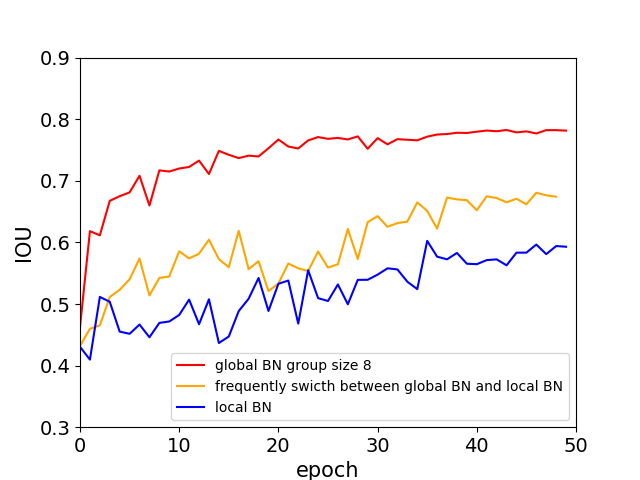
\includegraphics[width=7.5cm]{figure/switch-frequently.png}
    \caption{Training accuracy when switch between local BN and global BN frequently}
    \label{fig:switch-frequently}
\end{figure}

We further did an experiment in which the semantic image segmentation training process switches between local BN and global BN frequently. The accuracy improvement is shown in Figure~\ref{fig:switch-frequently}. Bad accuracy improvement from frequent switching between local BN and global BN indicates that our progressive design is reasonable.

Usually the number of available GPUs is a power of 2, so we double the group size $X_i$ in each epoch so that we can balance the number of GPUs in each group. Based on the simplification, our problem can be represented as:

\begin{align}
  \text{minimize} &\null \sum_{i=1}^{k_1} t(1) + \sum_{i=k_1}^{k_2} t(2) + \sum_{i=k_2}^{k_3} t(4) \dots +\sum_{i=k_j}^{n} t(N) \\
  \text{subject to} &\null \sum_{i=1}^{k_1} \delta_{A_i}(1) + \sum_{i=k_1}^{k_2} \delta_{A_i}(2) + \dots +  \sum_{i=k_{j}}^{n} \delta_{A_i}(N) =  \sum_{i=1}^{n_0} \delta_{A_i}(N)
\end{align}


%So we suggest that $X_i$ should only increase from 1 to N gradually like how learning rate decays.
%We treat the group size 


%Semantic image segmentation is one of the deep learning application scenarios. We apply global batch normalization to DeepLab \cite{deeplab}, a commonly used model for semantic image segmentation task, and train our model based on Visual Object Class Challenge 2012 dataset(VOC2012) \cite{pascal-voc-2012},  We test it on 8 GTX 1080Ti graphics processors under mini batch size 2.


\begin{table}[]
    \centering
    \begin{tabular}{|c|c|}
         \hline Name & Description \\
         \hline \textit{gap} & a small constant threshold used to determine whether training has converged \\
         \hline    B_b & the bottleneck of the batch size in each group  \\
         \hline k &   number of history epochs used to determine whether training has converged \\
         \hline
    \end{tabular}
    \centering
    \newline
    \newline
    \caption{Parameters notation in progressive update algorithm}
    \label{tab:algo-notation}
\end{table}

Because we have to double 1 for $\log_2 N$ times to reach N, now we need to decide when to double the synchronization group size $X_i$. The complexity of our problem is dramatically reduced to an acceptable range. And we propose a Progressive Update Algorithm (Line 10 in Algorithm~\ref{algo:general}) to solve it. Table \ref{tab:algo-notation} shows the description of parameters used in this algorithm. 


%\subsection{Update Function}


\begin{algorithm}
    \caption{p-update function}
    \label{algo:update}
    \State \textbf{Parameter:}  k, gap, $B_b$
    \State \textbf{Input:} B, N, $X_{i-1}$, $A_{i-k}$, $A_i$
    \State \textbf{Output:} $X_i$
    \begin{algorithmic}[1]
        \State $B_g$ = $X_{i-1}$ * B / N
        \If{$B_g < B_b$}
            \If{$A_{i-1} -A_{i-k} < gap $}
                \State $X_i$ = $\min$ (2$X_{i-1}$, N)
            \Else 
                \State $X_i$ = $X_{i-1}$
            \EndIf
        \Else
            \State $X_i$ =$\max$ ($X_{i-1}$ /2, 1)
        \EndIf
    \end{algorithmic}
\end{algorithm}

%In Algorithm~\ref{algo:PBN-base}, we utilize an \textit{update} function (Line 10), as illustrated in Algorithm~\ref{algo:update}, to determine the synchronization group size for next training epoch. 

Theoretically speaking, training accuracy improvement reduce with training epochs increasing. The heuristic way to decide when to double synchronization group size is when the training tends to converge. Here we use the comparison between accuracy improvement in the past $k$ epochs and a small constant threshold which denotes as $gap$ to determine if the training tends to converge. This threshold is learned from previous training accuracy traces' fluctuation after they've converged. In addition, based on the fact that when mini batch size is large enough, data synchronization across GPUs is of little effect and will lead to additional cost. So group size $X_i$ should be reduced if the batch size in each group $B_g$ exceeds $B_b$ in order to avoid unnecessary extra cost. Detail of the progressive update algorithm (denoted as $p$-$update$ function) is presented in Algorithm~\ref{algo:update}.


\subsection{Stop Condition}

Note that we set an \textit{expected} accuracy as a constraint in problem formulation part to guide the general algorithm. However, when applied to deep neural networks training, we usually have no idea on the \textit{expected} accuracy and the stop condition (Line 4 in Algorithm~\ref{algo:general}) could not be satisfied. 

For example, in some cases, if the training accuracy does not improve after $K$ epochs, we will stop the training process. In other cases, the training process will not stop until the epoch reaches to a given value $E_{max}$. 
In our approach, we should be able to adapt to the different stop conditions. Usually, we consider the three stop conditions as shown in Table~\ref{tab:stop-condition}. In a training process, the users can select one stop condition from the three as they want.


\begin{table}[]
    \centering
    \begin{tabular}{|c|c|c|}
         \hline Stop Condition & Given Value& Description \\
         \hline Accuracy Condition & $A_{max}$ & $A_i \geq A_{max}$ \\
         \hline Epoch Condition &  $E_{max}$ & $i \geq E_{max}$  \\
         \hline Accuracy Improvement Condition  &  $K$ & $i \geq K$ and $ A_{i-K} \geq A_i$ \\
         \hline
    \end{tabular}
    \centering
    \newline
    \newline
    \caption{Stop Condition Descriptions}
    \label{tab:stop-condition}
\end{table}


%{\bf Accuracy Condition.} Given $A_{max}$ and the stop condition is (Line 4 in Algorithm~\ref{algo:general}):

%\begin{equation}
%    while\ (A_i < A_{max})
%\end{equation}

%{\bf Epoch Condition.} Given $E_{max}$ and the stop condition is:
%\begin{equation}
%    while\ (i < E_{max})
%\end{equation}

%{\bf Accuracy Improvement Condition.} Given $K$ and the stop condition is:
%\begin{equation}
%    while\ (i < K\ or\ A_i > A_{i-K})
%\end{equation}

%Our approach should 



\begin{algorithm}
    \caption{Progressive Batch Normalization Algorithm}
    \label{algo:PBN}
     \State \textbf{Parameter:} 
    \State    \quad   k, gap, $B_b$: progressive update parameters shown in Table~\ref{tab:algo-notation}
    \State    \quad   $Stop$ : stop condition shown in Table~\ref{tab:stop-condition}
    \State \textbf{Input:} 
    \State    \quad    dataset : training dataset 
    \State    \quad    eval\_data : data used in evaluation 
    \State    \quad    model : pre-trained model 
    \State    \quad    B : training batch size 
    \State    \quad    N : number of available GPUs
    
    \begin{algorithmic}[1]
        \State $A_0$ = eval(model, eval\_data)
        \State $X_0$ = 1
        \State i = 0
        \While {not $Stop$}
            \State \textbf{In epoch $i$:}
            \State \quad data = dataset.fetch(B)
            \State \quad model = train($X_i$, model, data) 
            \State $A_i$ = eval(model, eval\_data)
            \State i = i + 1
            \State $X_i$ = p-update(B, N, $X_{i-1}$,  $A_{i-k}$, $A_{i-1}$)
        \EndWhile
    \end{algorithmic}
\end{algorithm}

\subsection{Progressive Batch Normalization Algorithm}

%Usually ,  In this case, our PBN algorithm should be extended to adapt to the real scenario. 
Our Progressive Batch Normalization Algorithm is shown in Algorithm~\ref{algo:PBN}. In epoch $i$, we fetch the data from the dataset (Line 6) and train our model (Line 7) based on our selected group size $X_i$. After each epoch, we first evaluate the training accuracy $A_i$ (Line 8) and then determine the new group size $X_{i+1}$ (Line 10) based on the proposed progressive update algorithm shown in Algorithm~\ref{algo:update}. Finally, we check whether the stop condition is satisfied (Line 4). If not, we repeat the same loop.




%\subsection{Implementation Details}

%Apache MXNet\cite{chen2015mxnet} is a fast scalable training and inference framework which can distribute deep learning workloads across multiple GPUs with near-linear scalability. We apply Nvidia Collective Communication Library to Batch Normalization Operator in MXNet to synchronize key data like mean and variance. And enable changing synchronization group size during training process.


\section{Evaluations}


\subsection{Experimental Setup}
We utilize MXNet~\cite{chen2015mxnet} framework to train the deep neural network. 
We train our models on 8 GTX 1080Ti graphics cards under different batch sizes, where the default value $B$ is 16. We utilize the Epoch Condition as the stop condition, where $K$ is equal to 50. We select $gap=0.1$, $B_b=16$, $k=5$ and $K=10$.

{\bf Model and Dataset. }We apply our progressive batch normalization 
in training three different models with different datasets, including Resnet-20 model on Cifar10 dataset, Resnet-50 model on Cityscape dataset~\cite{cityscapes} and DeepLab model on VOC2012 dataset. 

{\bf Comparisons. } We utilize the Batch Normalization Algorithm, where group size is 1, as {\bf Baseline}. 
The global batch normalization algorithm, where the group size is equal to the number of available GPUs, is dented as {\bf GBN}. We denote our proposed algorithm as {\bf PBN} (short for progressive batch normalization).
We evaluate PBN in the flowing aspects, including training accuracy and training speed.


%We train our models on 8 GTX 1080Ti graphics cards under batch size 16, so mini batch size is 2 for each GPU. We compare the accuracy score and the total time used to train it among global batch normalization at largest group size 8, progressive batch normalization and local batch normalization. 



\subsection{Experimental Results}

% \begin{figure}[h]
% \begin{minipage}[t]{0.45\linewidth}
% \centering
% 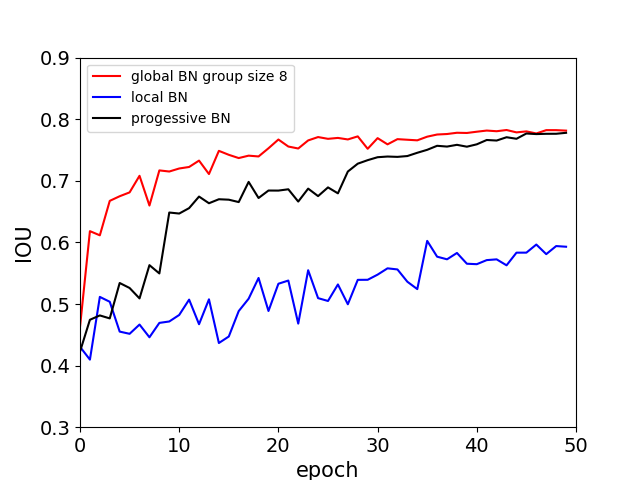
\includegraphics[width=1\textwidth]{figure/progressiveBN.png}
% \caption{DeepLab training trace on VOC2012 using progressive Batch Normalization}
% \label{fig:progressiveBN}
% \end{minipage}
% \hfill
% \begin{minipage}[t]{0.45\linewidth}
% \centering
% 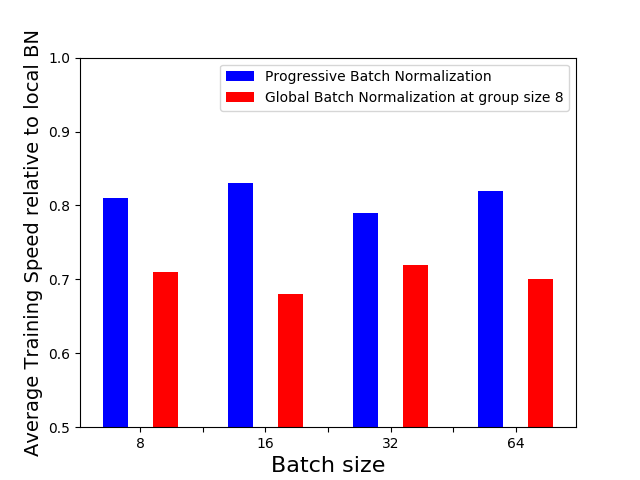
\includegraphics[width=1\textwidth]{figure/pbn-cifar10.png}
% \caption{Resnet-20 training speed improvement on Cifar10 between PBN and GBN algorithm}
% \label{fig:cifar10-PBN}
% \end{minipage}
% \end{figure}

\begin{figure}
    \centering
    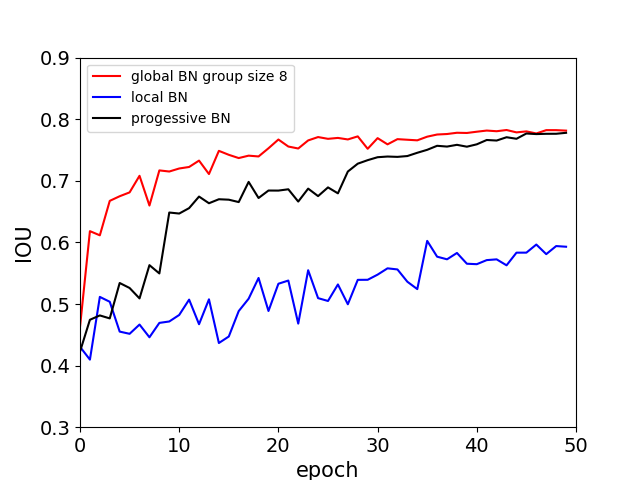
\includegraphics[width=7.5cm]{figure/progressiveBN.png}
    \caption{DeepLab training trace for different algorithms}
    \label{fig:progressiveBN}
\end{figure}


{\bf Training Accuracy Comparison.} Figure~\ref{fig:progressiveBN} shows the training trace for DeepLab model on VOC2012 dataset. We observe that PBN achieve almost the same IOU with GBN in the end (\textbf{77.8\%} and \textbf{78.1\%}).
Compared with  Baseline, PBN can obtain up to {\bf 35\%} accuracy improvement. %We obtain similar results in other datasets.

%From Figure~\ref{fig:progressiveBN} we can see, DeepLab with progressive batch normalization achieve an IOU of \textbf{77.8\%} in the end, while DeepLab with global batch normalization at largest group size 8 makes it to \textbf{78.1\%}. In Resnet-50 training on Cityscape datset, IOU score also reaches \textbf{64.8\%} compared to \textbf{64.9\%} achieved by global BN at largest group size 8. Our progressive batch normalization \textbf{almost} reaches a validation IOU score as good as global batch normalization at largest group size, and much better than local batch normalization. 

%\subsection{Training Performance}

{\bf Overall Performance Comparison. } Figure~\ref{fig:pbn-speed-improve} shows the overall performance improvement for different algorithms. Compared to using  GBN, PBN can obtain 10-20\% performance improvement 
in those three deep neural network training tasks. 

{\bf Performance Improvement in Different Batch Size. }
Figure~\ref{fig:cifar10-PBN} shows the performance improvement in different batch size from 8 to 64. We utilize Resnet-20 on Cifar10 dataset as an example. We observe that the speed improvement is also significant up to \textbf{18.4\%}.
%In addition, we test progressive batch normalization in  under different batch sizes from 8 to 64. 
%The speed improvement is also significant up to \textbf{18.4\%} in Figure~\ref{fig:cifar10-PBN}. 

{\bf Summary.} Based on these experiments, PBN indeed brings much speed improvement by reducing extra cost from unnecessary data synchronization. Besides, model training with less computational complexity tends to obtain more speed up with  PBN, because extra time cost from waiting for other GPUs in data synchronization process occupies a larger proportion in total training time, which means PBN can reduce more overhead from communication among GPUs.


\begin{figure}[h]
\begin{minipage}[t]{0.45\linewidth}
\centering
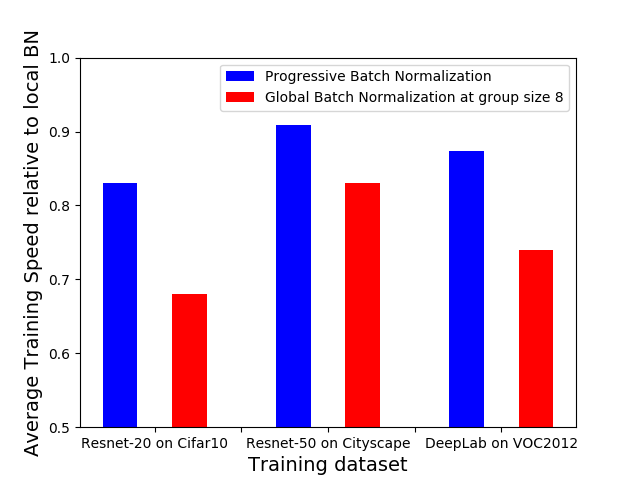
\includegraphics[width=1\linewidth]{figure/pbn-speed-improvement.png}
    \caption{Overall Performance Comparison in different datasets}
    \label{fig:pbn-speed-improve}
\end{minipage}
\hfill
\begin{minipage}[t]{0.45\linewidth}
\centering
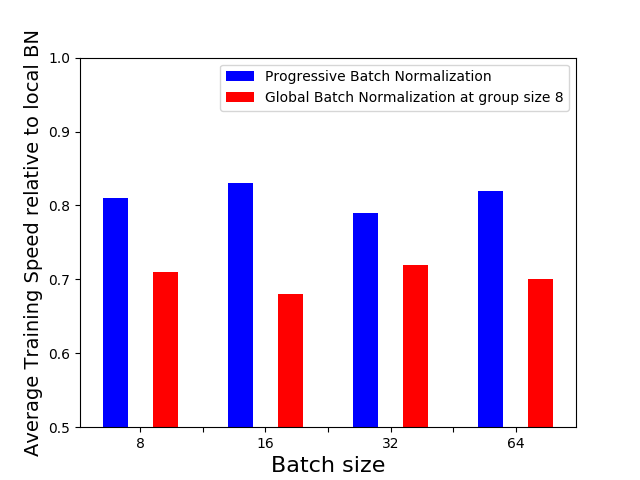
\includegraphics[width=1\textwidth]{figure/pbn-cifar10.png}
\caption{Performance improvement in different batch sizes}
\label{fig:cifar10-PBN}
\end{minipage}
\end{figure}


\section{Related work}

%Add more reference like GroupBN(kaiming he) GlobalBN(zhanghang) L1BN


There are also other work on optimization for Batch Normalization. Group Normalization \cite{groupBN} divides channels into groups and computes each group the mean and variance for normalization. Group Normalization's computation is independent of batch sizes, and its accuracy is table in a wide range of batch sizes.

Besides, L1-Norm \cite{L1BN} reduces additional computation and memory usage to linear cost in both the forward and backward propagation during training. L1-Norm is approximately equivalent to the original L2-Norm BN by multiplying a scaling factor and achieves good speedup with lower energy consumption.


\section{Conclusions}

Since the batch size of neural network is limited by the memory size of single device and original BN algorithm results in data-model coupled parallelism in multi-GPUs, we propose and implement Progressive BN algorithm to eliminate the training loss introduced by BN layer under multi-GPUs. This algorithm is adaptively deployed to balance the accuracy and efficiency. Experimental results show that our algorithm can get up to 18.4\% performance improvement over traditional methods without sacrificing the training accuracy. 

%For $N$ GPUs that mini-batch size equals to $BZ_{mini}$, we obtain the training accuracy  nearly equivalent to the result of single GPU that batch size equals to $N * BZ_{mini}$. 
%Under small batch size situation, our progressive batch normalization algorithm can bring much improvement to complex deep neural networks with acceptable speed loss.


%We will implement multi-machine global batch normalization for distributed machine learning cluster later. More work need to be done to optimize its performance.



\bibliographystyle{splncs03}
\bibliography{cited}



\end{document}